\chapter{Frequenze e tabelle}
\label{cha:frequenzeTabelle}
\begin{table}%[!t]
	\centering
	\begin{tabular} {*{2} {S[table-format=1.0]}S[table-format=1.2]*{2} {S[table-format=2.0]} }%{SSS[table-format=1.2]
		%S[table-format=2.0]S}
		\toprule
		{Voto}  & {Assoluta} & {Relativa} & {Percentuale} &{Cumulata} \\
		\midrule 
		1	& 2 & 0.15 & 15\% & 2  \\ 
		2	& 3 & 0.15 & 15\% & 5 \\ 
		3	& 1 & 0.05 & 5\% & 6 \\ 
		4	& 4 & 0.2 & 20\% & 10 \\ 
		5	& 2 & 0.1 & 10\% & 12 \\ 
		6 	& 2 & 0.1 & 10\% & 14 \\ 
		7	& 2 & 0.1 & 10\% & 16 \\ 
		8	& 1 & 0.05 & 5\% & 17 \\ 
		9	& 2 & 0.1 & 10\% & 19 \\ 
		10	& 0 & 0 & 0\% & 19 \\ 
		\bottomrule
	\end{tabular}
	\caption{Frequenze a confronto}
	\label{tab:FrequenzeConfronto}
\end{table}
\section{Frequenze}
\label{sec:Frequenze}
\subsection{Un esempio pratico}
\label{sec:Un esempioPratico}
Per parlare di statistica partiamo da un esempio pratico. Supponiamo di avere una classe di venti alunni. La~\vref{tab:alunnovoto1} riporta i risultati di una verifica. L'insieme dei dati costituisce una popolazione\index{Popolazione}. Una popolazione è formata da unità statistiche\index{Unità statistiche}, in questo caso sono i voti ma potrebbero essere misure, il numero di punti fatti da un giocatore di basket etc.   

Ciò  che  ci dice questa tabella non va oltre il semplice elenco dei risultasti. Non otteniamo un risultato migliore  considerando la~\vref{fig:VotiAlunni} associata alla tabella. In ordinata abbiamo i voti in ascissa i nomi degli alunni. Ma come è andata la prova per la classe? Per dare una prima risposta  definiamo il concetto di frequenza. 	La frequenza\index{Frequenza} di un dato indica quante volte quel valore di ripete nel campione.
%\begin{defn}[Frequenza]
%	La frequenza\index{Frequenza} si un dato indica quante volte quel valore di ripete nel campione.
%\end{defn}
 \begin{table}
	\centering
	\begin{tabular}{*{2}{S[table-format=1.0]}S[table-format=2.0] S[table-format=1.0]}
\toprule
	{Alunno}	& {Voto}&{Alunno}	& {Voto} \\
\midrule 
	1	& 5 &11 & 1\\ 
	2	& 7 &12 & 6 \\ 
	3	&  2&13 & 3 \\ 
	4	&  4&14 & 7\\ 
	5	&  2&15 & 8\\ 
	6	& 6 &16 & 2\\ 
	7	& 4 &17 & 1\\ 
	8	& 4 &18 & 4\\ 
	9	& 5 &19 & 1\\ 
	10	& 9 & 20& 9\\ 
\bottomrule 
	\end{tabular} 
	\caption{Alunno voto}
	\label{tab:alunnovoto1}
\end{table}
\begin{figure}
	\centering
	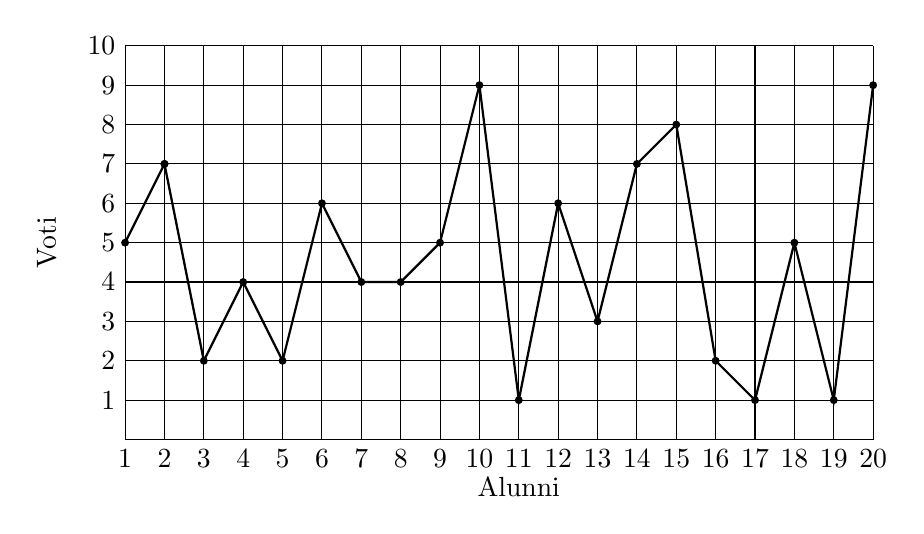
\begin{tikzpicture}[scale=0.5]
	\draw[mark=*,thick] plot coordinates{(1,5) (2,7) (2,7) (3,2)
		(4,4) (5,2) (6,6) (7,4) (8,4) (9,5) (10,9)(11,1) (12,6)(13,3)(14,7)(15,8)(16,2)(17,1)(18,5)(19,1)(20,9)};
	\draw (1,0) grid (20,10);
	\foreach \y in {1,2,...,10} \draw(1,\y)node[left]{\y};
	\foreach \x in {1,2,...,20} \draw(\x,0)node[below]{\x};
	\draw (11,-1.2) node{Alunni};
	\draw (-1,5) node[rotate=90]{Voti};
	\end{tikzpicture}
	\caption{Voti e Alunni}
	\label{fig:VotiAlunni}
\end{figure}
\subsection{Frequenze assolute}
%Un primo tipo di frequenza è quella assoluta.
\begin{defn}[Frequenza assoluta]
	La frequenza assoluta\index{Frequenza!assoluta} è il numero di volte in cui un'unità statistica compare in una popolazione.
\end{defn}Guardando la tabella vediamo che la frequenza assoluta del voto ``cinque'' è due perché  nella~\vref{tab:alunnovoto1} il voto ``cinque'' compare due volte. La~\vref{tab:FrequenzeAssolute} rappresenta le frequenze assolute dei voti della verifica. 

La tabella riassume la~\vref{tab:alunnovoto1} ponendo accanto ad ogni voto la sua frequenza assoluta.  Ovviante la somma delle frequenze è uguale al numero degli alunni della classe o,  in generale, al numero degli elementi della popolazione.  Il grafico a barre nella~\vref{fig:FrequanzeAssoluteVoti} mostra l'andamento delle frequenze.

Leggendo il grafico è evidente che la verifica non è andata molto bene dato che tredici alunni sono sotto la sufficienza. 
%\begin{table}
%	\centering
%	\begin{tabular}{SS}
%		\toprule
%		{Voto}&{Frequenza}  \\
%		\midrule 
%		1& 3 \\ 
%		2& 3 \\ 
%		3&  1\\ 
%		4&  4\\ 
%		5&  2\\ 
%		6&  2\\ 
%		7&  2\\ 
%		8&  1\\ 
%		9&  2\\ 
%		10&  0\\
%		\midrule
%		{Totale}&  20\\ 
%	\bottomrule
%	\end{tabular} 
%	\caption{Frequenze assolute}
%	\label{tab:FrequenzeAssolute}
%\end{table}
\begin{figure}
	\centering
	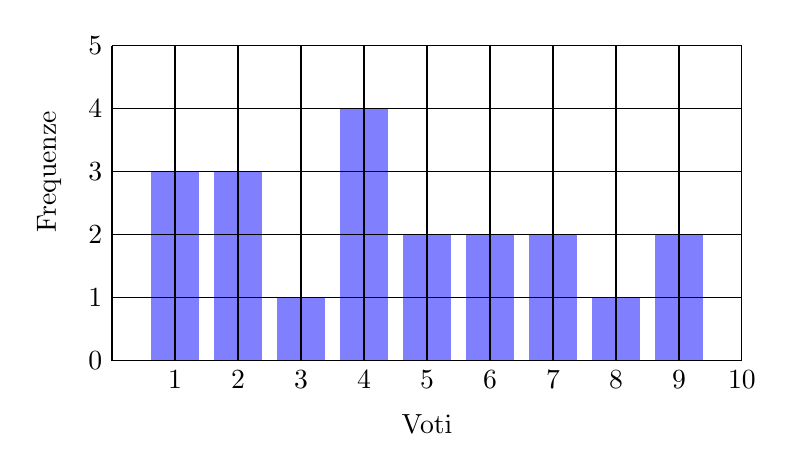
\begin{tikzpicture}[scale=0.8]
	\draw[line width=6mm,color=blue!50] plot[ycomb] coordinates{(1,3) (2,3) (3,1) (4,4)
		(5,2) (6,2) (7,2) (8,1) (9,2) (10,0)};
	\draw (0,0) grid (10,5);
	\foreach \y in {0,1,...,5} \draw(0,\y)node[left]{\y};
	\foreach \x in {1,2,...,10} \draw(\x,0)node[below]{\x};
	\draw (5,-1) node{Voti};
	\draw (-1,3) node[rotate=90]{Frequenze};
	\end{tikzpicture}
	\caption{Frequenze assolute}
	\label{fig:FrequanzeAssoluteVoti}
\end{figure}
\subsection{Frequenza relativa e percentuale}
Il maggior problema di una frequenza assoluta è che non consente un confronto fra campioni che non hanno lo stesso numero di unità statistiche. Continuando con l'esempio dei voti, se ho un'altra  classe di quindici alunni come faccio a confrontare i risultati ottenuti? Bisogna introdurre un altro tipo di frequenza: la frequenza relativa.\index{Frequenza!relativa} 
\begin{defn}[Frequenza relativa]
La frequenza relativa è la singola frequenza assoluta divisa per il numero totale delle unità statistiche. 
\end{defn}
In questo caso, per costruire la~\vref{tab:FrequenzeRelative}, dividiamo ogni frequenza della~\vref{tab:FrequenzeAssolute} per il numero totale dei voti nella classe cioè venti. La~\vref{tab:FrequenzaRelativaExcel} mostra come organizzare i calcoli.  Da  notare come, in questo caso,  la somma delle frequenze relative sia uno. 

La~\vref*{fig:FrequenzeRelative} è un diagramma ``a torta'' che rappresenta le frequenze relative dei voti nella classe.
\begin{table}
	\begin{subtable}[b]{.5\linewidth}
		\centering\begin{tabular}{*{2}{S[table-format=1.0]}}
			\toprule
			{Voto}&{Frequenza}  \\
			\midrule 
			1& 3 \\ 
			2& 3 \\ 
			3&  1\\ 
			4&  4\\ 
			5&  2\\ 
			6&  2\\ 
			7&  2\\ 
			8&  1\\ 
			9&  2\\ 
			10&  0\\
			\midrule
			{Totale}&  20\\ 
			\bottomrule
		\end{tabular}
		\caption{Frequenze assolute}\label{tab:FrequenzeAssolute}
	\end{subtable}%
	\begin{subtable}[b]{.5\linewidth}
		\centering\begin{tabular}{S[table-format=2.0]S[table-format=1.2]}
			\toprule
			{Voto}&{Frequenza}  \\
			\midrule 
			1& 0.15 \\ 
			2& 0.15 \\ 
			3&  0.05\\ 
			4&  0.2\\ 
			5&  0.1\\ 
			6&  0.1\\ 
			7&  0.1\\ 
			8&  0.05\\ 
			9&  0.1\\ 
			10& 0.0\\
			\midrule
			{Totale}&  1\\ 
			\bottomrule
		\end{tabular}
		\caption{Frequenze relative}\label{tab:FrequenzeRelative}
	\end{subtable}
 	\caption{Frequenze}
	\label{fig:subFrequenze}
\end{table}
\begin{figure}
	\centering
	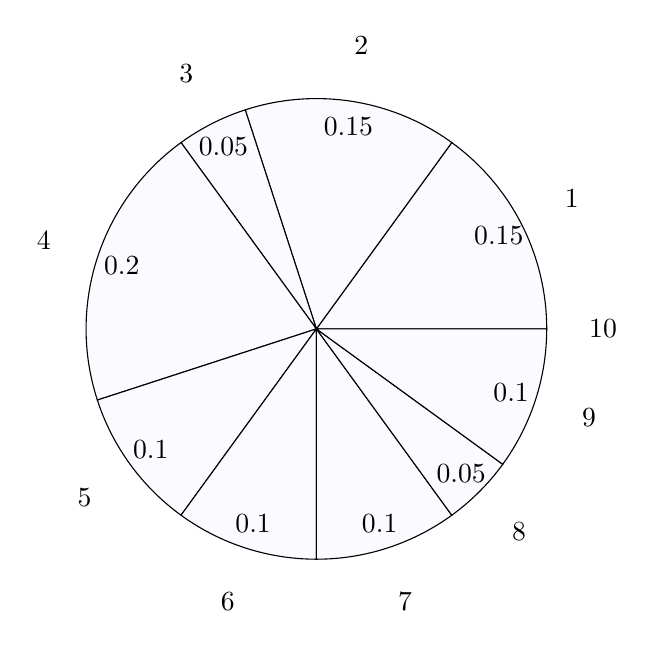
\begin{tikzpicture}[scale=0.65]
	\draw[fill=black!2!blue!2] (0,0)--(0:4.5)arc(0:54:4.5)--cycle;
	\draw ({(54)/2}:4) node {\num{0.15}};
	\draw ({(54)/2}:5.6) node {\num{1}};
	\draw[fill=black!2!blue!2] (0,0)--(54:4.5)arc(54:108:4.5)--cycle;
	\draw ({(54+108)/2}:4) node {\num{0.15}};
	\draw ({(54+108)/2}:5.6) node {\num{2}};
	\draw[fill=black!2!blue!2] (0,0)--(108:4.5)arc(108:126:4.5)--cycle;
	\draw ({(108+126)/2}:4) node {\num{0.05}};
	\draw ({(108+126)/2}:5.6) node {\num{3}};
	\draw[fill=black!2!blue!2] (0,0)--(126:4.5)arc(126:198:4.5)--cycle;
	\draw ({(126+198)/2}:4) node {\num{0.2}};
	\draw ({(126+198)/2}:5.6) node {\num{4}};
	\draw[fill=black!2!blue!2] (0,0)--(198:4.5)arc(198:234:4.5)--cycle;
	\draw ({(198+234)/2}:4) node {\num{0.1}};
	\draw ({(198+234)/2}:5.6) node {\num{5}};
	\draw[fill=black!2!blue!2] (0,0)--(234:4.5)arc(234:270:4.5)--cycle;
	\draw ({(234+270)/2}:4) node {\num{0.1}};
	\draw ({(234+270)/2}:5.6) node {\num{6}};
	\draw[fill=black!2!blue!2] (0,0)--(270:4.5)arc(270:306:4.5)--cycle;
	\draw ({(270+306)/2}:4) node {\num{0.1}};
	\draw ({(270+306)/2}:5.6) node {\num{7}};
	\draw[fill=black!2!blue!2] (0,0)--(306:4.5)arc(306:324:4.5)--cycle;
	\draw ({(306+324)/2}:4) node {\num{0.05}};
	\draw ({(306+324)/2}:5.6) node {\num{8}};
	\draw[fill=black!2!blue!2] (0,0)--(324:4.5)arc(324:360:4.5)--cycle;
	\draw ({(324+360)/2}:4) node {\num{0.1}};
	\draw ({(324+360)/2}:5.6) node {\num{9}};
	\draw ({(0}:5.6) node {\num{10}};
	\end{tikzpicture}
	\caption{Frequenze relative}
	\label{fig:FrequenzeRelative}
\end{figure}
Una variante della frequenza relativa è la frequenza percentuale.\index{Frequenza!percentuale}
\begin{defn}[Frequenza percentuale]
	Otteniamo  la frequenza percentuale  scrivendo in forma percentuale la frequenza relativa. 
\end{defn} 
La frequenza percentuale del voto ``tre''  è $5\%$. 
\begin{figure}[!ht]
	\centering
	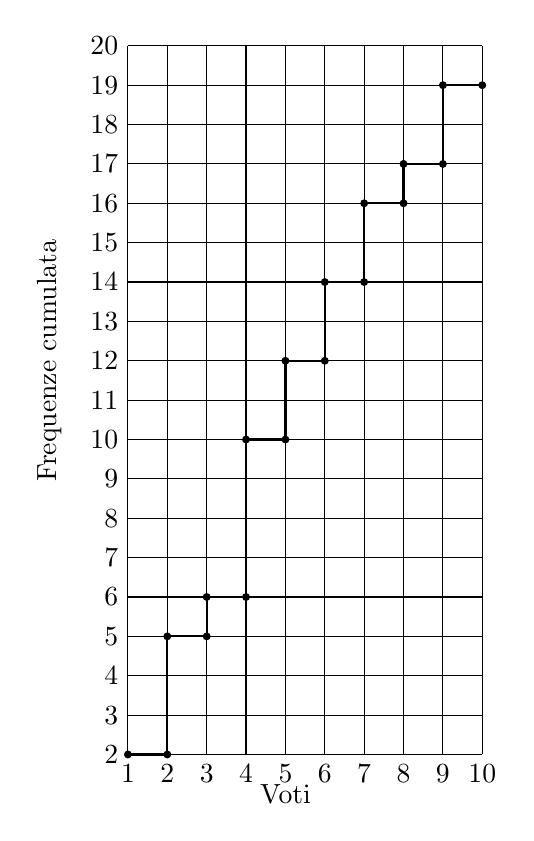
\begin{tikzpicture}[scale=0.5]
	\draw[mark=*,thick] plot coordinates{(1,2)(2,2) (2,5) (3,5)(3,6)(4,6) (4,10)(5,10)
		(5,12)(6,12) (6,14)(7,14) (7,16) (8,16) (8,17)(9,17) (9,19) (10,19)};
	\draw (1,2) grid (10,20);
	\foreach \y in {2,3,...,20} \draw(1,\y)node[left]{\y};
	\foreach \x in {1,2,...,10} \draw(\x,2)node[below]{\x};
	\draw (5,1) node{Voti};
	\draw (-1,12) node[rotate=90]{Frequenze cumulata};
	\end{tikzpicture}
	\caption{Frequenza Cumulata}
	\label{fig:FrequenzaCumulata}
\end{figure}
\subsection{Frequenze cumulate}
Problema come conoscere il numero dei ragazzi che hanno ottenuto una valutazione inferiore ad un dato valore? Per rispondere a questa domanda introduciamo un nuovo concetto, quello di frequenza cumulata.
\begin{defn}[Frequenza cumulata]
	La frequenza cumulata\index{Frequenza!cumulata!assoluta} di una data unità è pari alla sua frequenza assoluta più la somma di tutte quelle che la  precedono.\[F_{i}=\sum_{i=1}^{i}n_{i}\]
\end{defn}
La~\vref*{fig:FrequenzaCumulata} mostra l'andamento della frequenza cumulata per il nostro esempio. La~\vref{tab:FrequenzaCumulataExcel} mostra come ottenere l'esempio.

La~\vref{tab:FrequenzeConfronto} riepiloga quanto detto in precedenza confrontando fra loro i vari risultati. Per ottenere tale tabella si può utilizzare un foglio elettronico come quello~\vpageref[foglio]{tab:FrequenzeaConfrontoExcel}
\begin{defn}[Frequenza relativa cumulata]
	La frequenza cumulata\index{Frequenza!cumulata!relativa} di una data unità è pari alla sua frequenza assoluta più la somma di tutte quelle che la  precedono.\[F_{i}/n=\dfrac{1}{n}\sum_{i=1}^{i}n_{i}\]
\end{defn}
 
 